%Centralizar verticalmente.
\newenvironment{midpage}{\vspace*{\fill}}{\vspace*{\fill}}
%Centralizar horizontalmente.
\newenvironment{midline}{\hspace*{\fill}}{\hspace*{\fill}}
\documentclass[12pts]{article}
\usepackage[utf8]{inputenc}
%Pacote para colocar cor no código.
\usepackage{color}
\definecolor{light-gray}{gray}{0.95}
%Pacote para inserir código.
\usepackage{listings}
\lstset{
    numbers=left,
    tabsize=2,
    backgroundcolor=\color{light-gray},
}
\title{
	Prática de Eletrônica Digital 1 - (119466)
	\singlespacing
		Turma E (Unb - Gama)
	\singlespacing
	\begin{midpage}
	\begin {large}
		Pré-Relatório Experimento 4
		\singlespace
    Circuitos Codificadores
	\end {large}
	\end{midpage}
}
\date{Setembro 11, 2016}
\usepackage{indentfirst}
\usepackage{setspace}
\usepackage{verbatim}
\usepackage[pdftex]{hyperref}
\usepackage{graphicx}
\begin{document}
\maketitle	
%\vspace{100 mm}
\begin{center}

\begin{tabular}{|c|l|r|}
\hline
Nome & Matrícula & Assinatura\\
\hline
Arthur Temporim & 140016759 & \\
\hline	
Eduardo Nunes & 140056149 & \\
\hline	
\end{tabular}

\end{center}

\pagebreak

\section{Pesquisa bibliográfica}

Três tipos de somadores são utilizados com maior frequência. O meio somador, somador completo e somador completo paralelo.
	
O circuito meio somador é constituído por duas entradas, que são os dois bits a serem somados, uma saída, que é a resposta da soma, e o carry para a próxima posição. Para construí-lo, utilizamos a tabela verdade com essas quatro variáveis. 

\begin{center}
	\begin{tabular}{|r|r|r|r|}
		\hline
		A & B & S & Cout \\
		\hline
		0 & 0 & 0 & 0 \\				
		\hline
		0 & 1 & 1 & 0 \\
		\hline
		1 & 0 & 1 & 0 \\
		\hline
		1 & 1 & 0 & 1 \\
		\hline
	\end{tabular}
\end{center}

Podemos obsevar que a saída S é exatamente idêntica a uma por XOR entre A e B. e Cout é uma porta AND entre A e B. Assim, 

\begin{figure}[!htb]
  \centering
  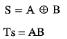
\includegraphics[scale=0.8	]{imagens/1}
  \label{figRotulo}
\end{figure}

O circuito meio somado recebe esse nome pois não consegue fazer uma soma com números de dois bits com apenas um circuito. São necessários dois circuitos somadores por bit.  Pois, esse circuito tem a saída para o carry, porém, não tem a entrada para ele. É necessário acoplar outro circuito para fazer a soma do carry. Visto esse problema, foi desenvolvido o somador completo, que tem uma entrada para o carry e consegue fazer somas com um circuito por bit. Conseguimos encontrar o circuito do somador completo através da tabela verdade de uma soma.

\begin{figure}[!htb]
  \centering
  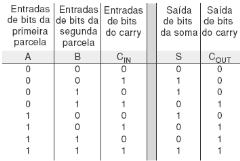
\includegraphics[scale=0.6	]{imagens/2}
  \label{figRotulo}
\end{figure}


Utilizando as simplificações, podemos perceber que as saídas S e Cout tem o seguinte resultado:

\begin{figure}[!htb]
  \centering
  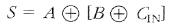
\includegraphics[scale=0.6	]{imagens/3}
  \label{figRotulo}
\end{figure}

\begin{figure}[!htb]
  \centering
  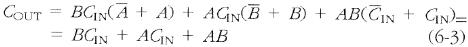
\includegraphics[scale=0.6	]{imagens/4}
  \label{figRotulo}
\end{figure}

\newpage
Assim, o circuito somador completo é representado pela simbologia a seguir.

\begin{figure}[!htb]
  \centering
  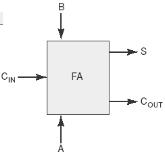
\includegraphics[scale=0.6	]{imagens/5}
  \label{figRotulo}
\end{figure}


Dessa maneira, é possível calcular a soma das entradas e do carry para um bit.
Para somar vários bits, são colocados vários SC em paralelo, um circuito por bit. A ligação pode ser observada a seguir.

\begin{figure}[!htb]
  \centering
  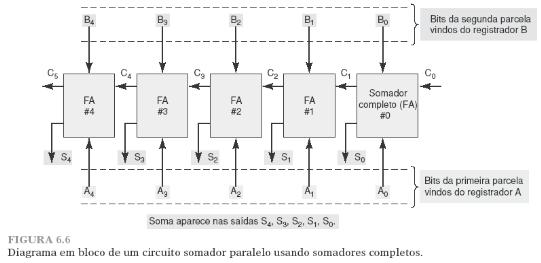
\includegraphics[scale=0.6	]{imagens/6}
  \label{figRotulo}
\end{figure}

Para executar a subtração dos números, seria necessário o mesmo procedimento que foi feito com os somadores, o que dobraria o número de circuitos. Para evitar esse excesso de portas, foi desenvolvido um sistema, chamado complemento de 2, que faz uma transformação no número, tornando-o diferente. Esse número modificado, sempre que for somado a outro número, será tido como negativo. Ou seja, seu quisermos fazer a operação A - B, devemos aplicar o complemento de 2 no número B, tornando-o -B e somando-o a A. O resultado estará correto.
A transformação do número em complemento de 2(CP2) é feita em duas etapas. Na primeira é feito o complemento de 1(CP1) , onde todos os bits do número são invertidos, por exemplo o 100. Ao aplicarmos CP1 temos 001. O resultado do CP1 é somado ao número 1, resultando assim o CP2. Portanto, temos que o CP2 de 100 é 010.

\newpage

\section{Projetos e Simulações}
\subsection{Projeto1 - Complemento de 1}
\subsubsection{Diagramas}

\textbf{Diagrama alto nível:}

\begin{figure}[!htb]
  \centering
  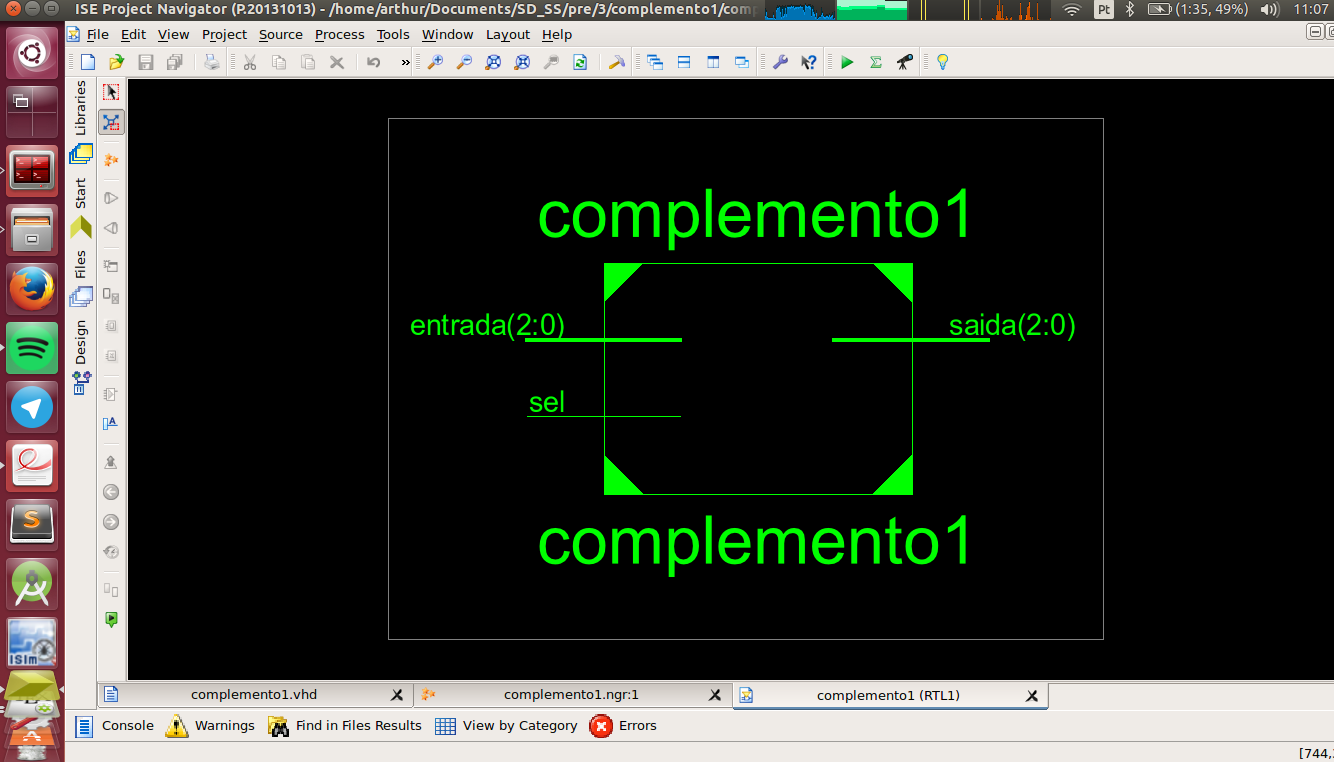
\includegraphics[scale=0.3	]{imagens/complementoSc1}
  \caption{Diagrama 1 - Ise Design Suit 14.7}
  \label{figRotulo}
\end{figure}

\newpage
\textbf{Diagrama 2 }

\begin{figure}[!htb]
  \centering
  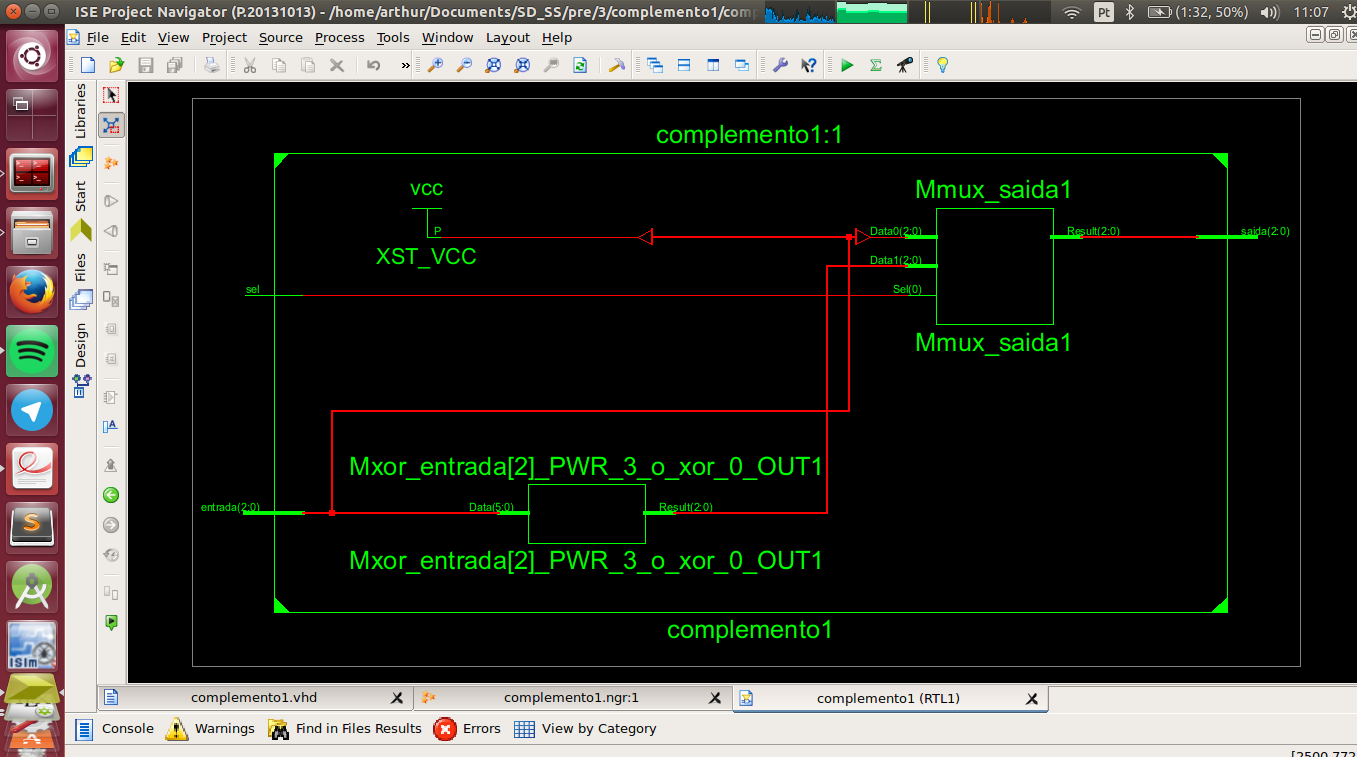
\includegraphics[scale=0.3	]{imagens/complementoSc2}
  \caption{Diagrama 2 - Ise Design Suit 14.7}
  \label{figRotulo}
\end{figure}


\subsubsection{Plano de validação}

Para Assegurar que o circuito está com o comportamento correto foram feitos os seguinstes testes:

\begin{center}
	\begin{tabular}{|r|r|r|}
		\hline
		Entrada & sel & saida \\
		\hline
		000 & 1 & 111 \\
		\hline
		000 & 0 & 000 \\
		\hline
	\end{tabular}
\end{center}

\newpage
\subsubsection{Código VHDL}

\lstinputlisting[language=vhdl]{complemento1/complemento1.vhd}

\newpage
\subsubsection{Forma de onda}

\textbf{Forma de onda gerada pelo circuito.}

\begin{figure}[!htb]
  \centering
  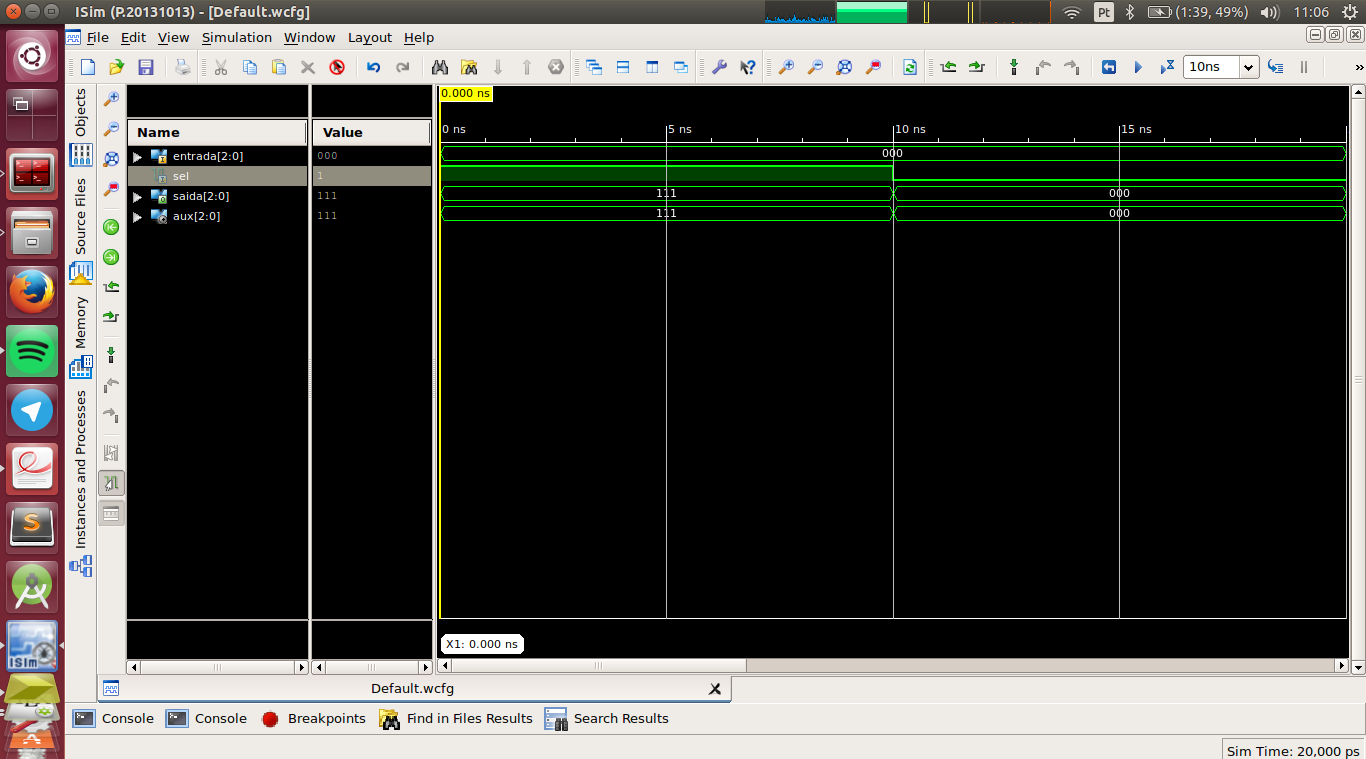
\includegraphics[scale=0.3	]{imagens/complemento1}
  \caption{Forma de onda - Ise Design Suit 14.7}
  \label{figRotulo}
\end{figure}

\newpage
\subsection{Projeto3 - Somador/Subtrator 3 bits}
\subsubsection{Diagramas}

\textbf{Diagrama alto nível:}

\begin{figure}[!htb]
  \centering
  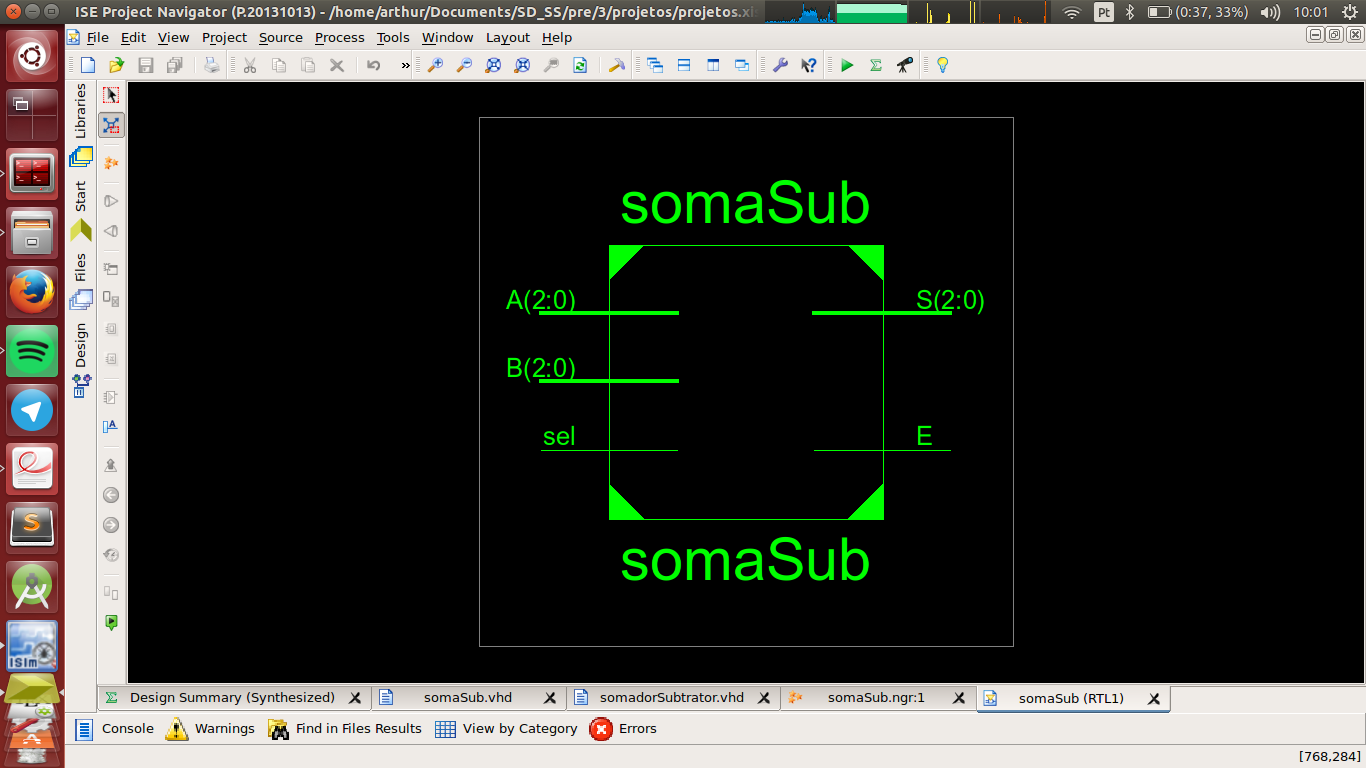
\includegraphics[scale=0.3	]{imagens/somaSub1}
  \caption{Diagrama 1 - Ise Design Suit 14.7}
  \label{figRotulo}
\end{figure}

\newpage
\textbf{Diagrama 2 }

\begin{figure}[!htb]
  \centering
  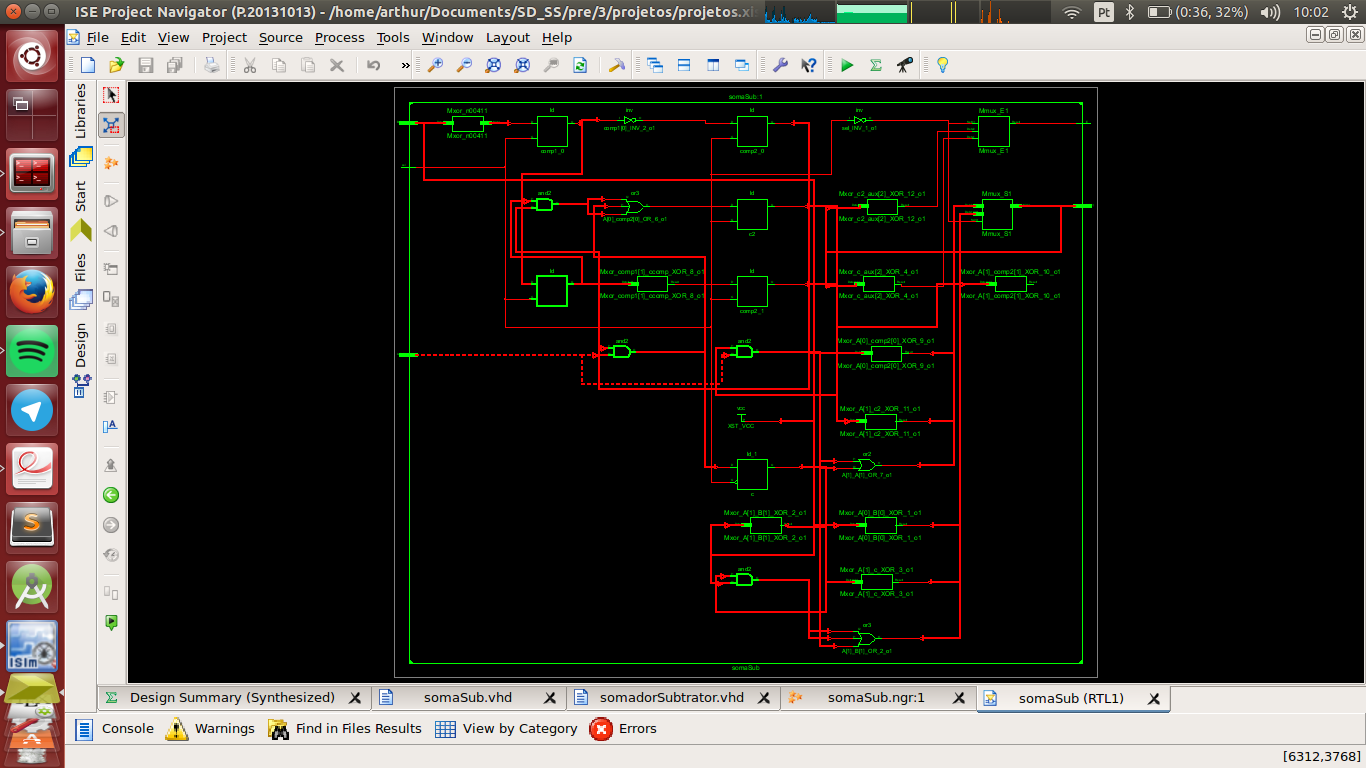
\includegraphics[scale=0.3	]{imagens/somaSub2}
  \caption{Diagrama 2 - Ise Design Suit 14.7}
  \label{figRotulo}
\end{figure}


\subsubsection{Plano de validação}

Para assegurar que o circuito está com o comportamento correto foram feitos os seguinstes testes:

\begin{center}
	\begin{tabular}{|r|r|r|r|r|}
		\hline
		Entrada1 & Entrada2 & Sel & Saida & Overflow\\
		\hline
		001 & 001 & 0 & 010 & 0\\
		\hline
		010 & 001 & 1 & 001 & 0\\
		\hline
		011 & 001 & 0 & 100 & 1\\
		\hline
	\end{tabular}
\end{center}

\newpage
\subsubsection{Código VHDL}

\lstinputlisting[language=vhdl]{projetos/somaSub.vhd}

\newpage
\subsubsection{Forma de onda}

\textbf{Forma de onda gerada pelo circuito. SOMA:}

\begin{figure}[!htb]
  \centering
  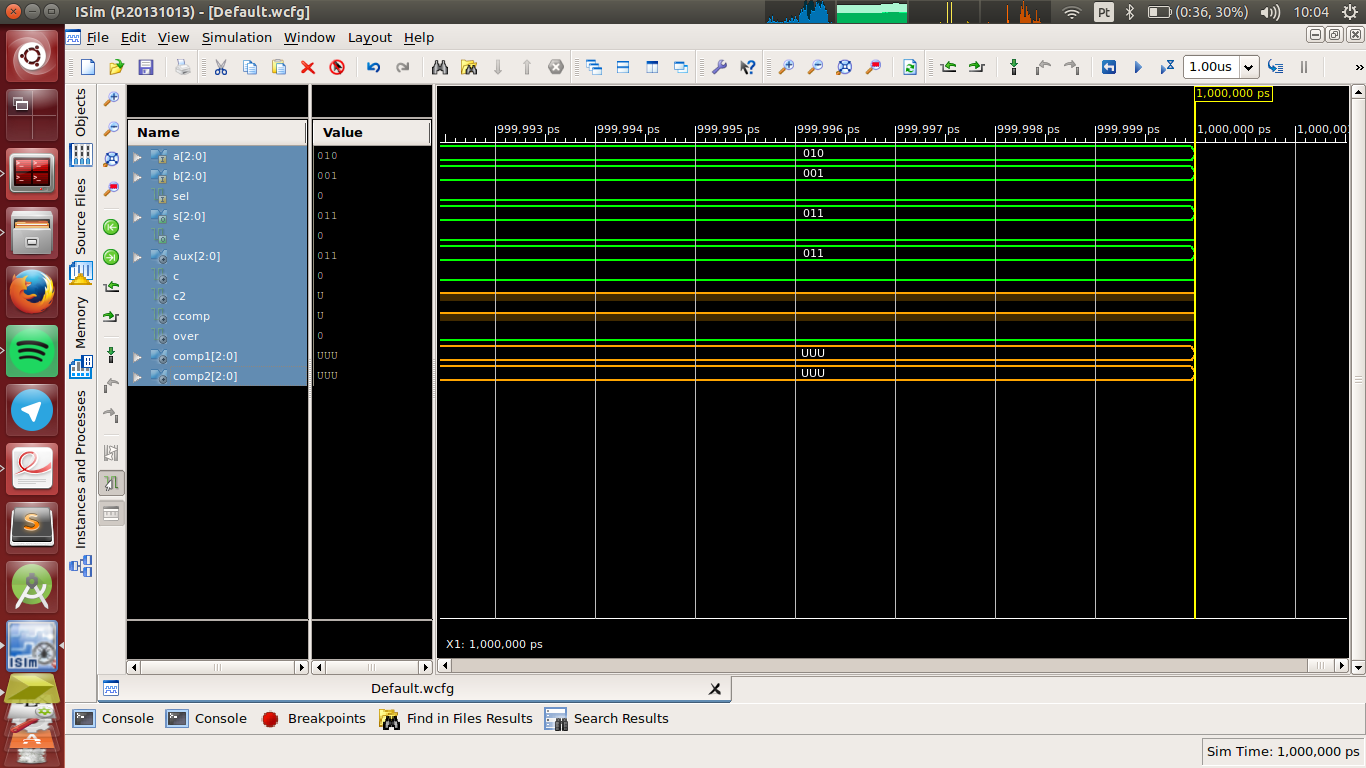
\includegraphics[scale=0.3	]{imagens/soma}
  \caption{Forma de onda - Ise Design Suit 14.7}
  \label{figRotulo}
\end{figure}

\newpage
\textbf{SUBTRAÇÃO:}
\begin{figure}[!htb]
  \centering
  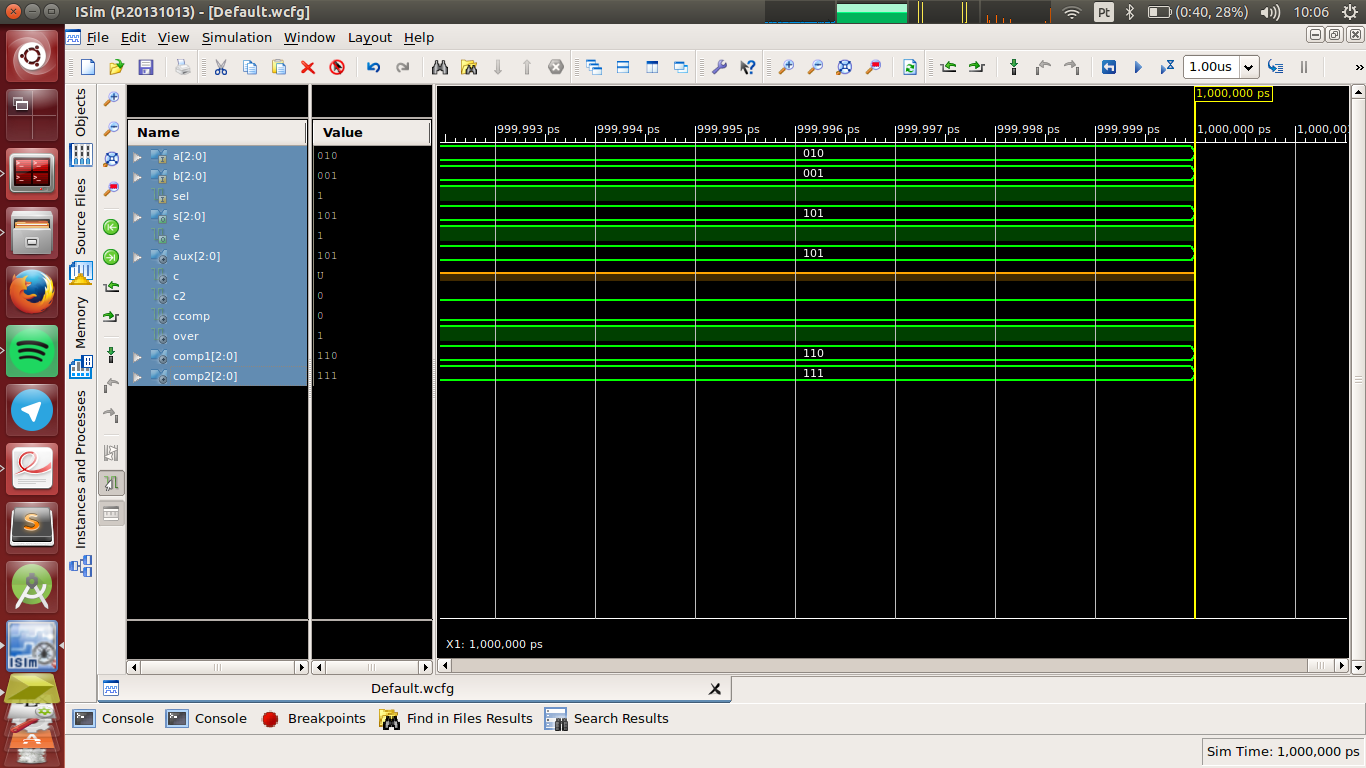
\includegraphics[scale=0.3	]{imagens/sub}
  \caption{Forma de onda - Ise Design Suit 14.7}
  \label{figRotulo}
\end{figure}

\newpage
\textbf{OVERFLOW:}
\begin{figure}[!htb]
  \centering
  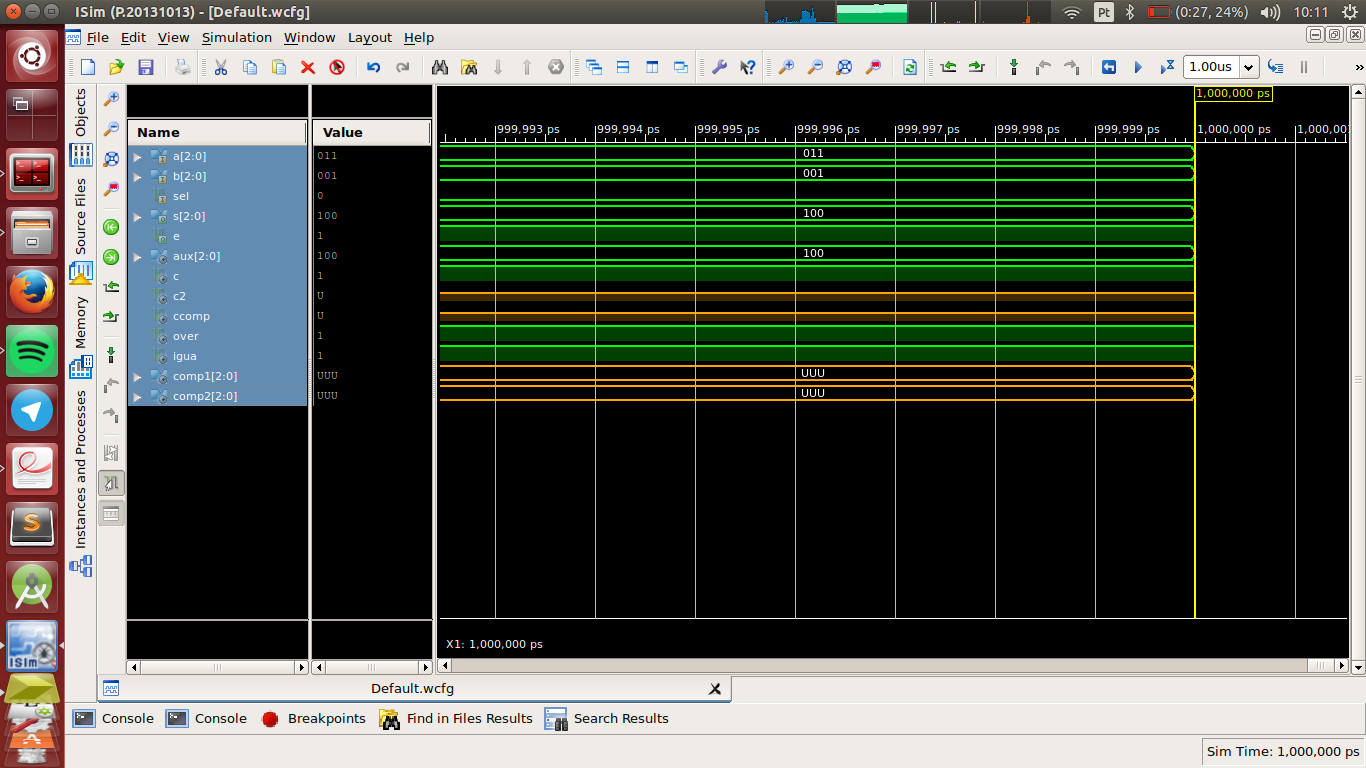
\includegraphics[scale=0.3	]{imagens/overflow}
  \caption{Forma de onda - Ise Design Suit 14.7}
  \label{figRotulo}
\end{figure}
\end{document}
